\chapter{3D case}

% {{{1 PROBLEM
\section{Problem}

In this part, we will be interested in doing the same work in 3D as in 2D except
that we will use a convex polyhedron instead of an euclidean ball in the
Minkowski sum. This will allow us to construct an anisotropic flow where the
flow will have different effects depending on the direction, like the normals of
the chosen convex polyhedron or not.

This choice will raise a number of issues such as the construction of the
Voronoi diagram of a point set under a polyhedral norm and the computation of
the volume of the intersection of a Voronoi cell and a convex polyhedron.

% {{{1 POLYHEDRAL NORM
\section{Polyhedral norm}
A polyhedral norm is a norm $ N $ defined as the following:

$$ \forall x \in \mathbb{R}^d,~ N(x) = \max_{i} (x | v_i) $$

where the $ v_i $ are given vectors from $ \mathbb{R}^d $.

This definition implies that the unit ball for the norm $ N $ is a polyhedron.
Indeed, if $ x \in B_N(0, 1) $, then :

$$ N(x) \leq 1 \Longleftrightarrow \forall i, (x | v_i) \leq 1 $$

So, the unit ball is defined by linear constraints. Thus, it is an intersection
of halfspaces and so is a convex polyhedron $ K $. Hence, computing the $ r $-offset
of a point cloud under a polyhedral norm $ N $ is the same as computing the
Minkowski sum (see the definition \ref{def:minkowski-sum}) of a point cloud and $ K $.

Conversely, if the convex polyhedron $ K $ is given then the vectors $ v_i $
previously defined are the outwards normals of the facets of $ K $.

We will denote by $ B_K(0, 1) $ the unit ball defined by the convex polyhedron $ K $.

% {{{1 CONSTRUCTION OF THE VORONOI DIAGRAM FOR A POLYHEDRAL NORM
\section{Construction of the Voronoi diagram for a polyhedral norm}

The main problem of a polyhedral norm is that the underlying Voronoi diagram is
not a partition of the space anymore.

For example, if we consider the $ L_\infty $ norm in the plane and two aligned
points, we have the following Voronoi diagram:

% TODO: insert figure

% {{{2 SYMBOLIC PERTURBATION
\subsection{Symbolic perturbation}

Given a polyhedral norm $ N $, we define its symbolic perturbation $ N_\epsilon
$ by: $ N_\epsilon (x) = N + \epsilon || x || $ where $ || \cdot || $ is an
euclidean norm (typically an $ L_p $ norm where $ 1 \leq p \leq +\infty $).

Then, we will show that the Voronoi cell of a point $ x $ under the norm $
N_\epsilon $ converges (when $ \epsilon \rightarrow 0 $) towards the Voronoi
cell defined as the following:

$$ V_{N'}(x, X) = \{ y \in \mathbb{R}^d,~\forall x' \in X,~N(x - y) \leq N(x'
-y) \text{ or } (N(x - y) = N(x' - y) \text { and } || x -y || \leq || x' - y ||) \} $$

First, we define the convergence of a set $ A $ towards another set $ B $: we
say that $ A $ converges towards $ B $ if the Hausdorff distance of $ A $ and $
B $ converges towards $ 0 $.

We recall that the Hausdorff distance is defined as follows:

$$ d_H(A, B) = \min \{ r \geq 0,~X \subset Y^{\oplus r} \text{ and } Y \subset
X^{\oplus r} \} $$

Now, we prove that $ V_{N_\epsilon}(x, X) $ converges towards $ V_{N'}(x, X) $
under the Hausdorff distance.

We want to prove that $ d_H(V_{N_\epsilon}(x, X), V_{N'}(x, X)) \rightarrow 0 $
Let us take a $ \delta > 0 $, we want to find $ \epsilon_\delta $ such that if $
\epsilon \leq \epsilon_\delta $ then $ d_H(V_{N_\epsilon}(x, X), V_{N'}(x, X))
\leq \delta $. The last inequality is equivalent to say that:
\begin{align}
    V_{N'}(x, X)) \subset V_{N_\epsilon}(x, X)^{\oplus \delta} \\
    V_{N_\epsilon}(x, X) \subset V_{N'}(x, X)^{\oplus \delta}
    \label{eqn:haussdorf-voronoi1}
\end{align}

Let us take care of the first inclusion:
% TODO: proof

And now the second inclusion:
Let us take $ y \in V_{N_\epsilon}(x, X) $. By definition of $ N_\epsilon $, we
have: $ \forall x' \in X,~N(x - y) + \epsilon || x - y || \leq N(x' - y) +
\epsilon || x' - y || $. If we choose $ z = y $ then $ z $ satisfies $ || z - y
|| \leq \delta $ and $ z \in V_{N'}(x, X) $. Indeed, using the previous
inequality, there are two cases: either $ N(x - y) \leq N(x' - y) $ or $ N(x -
y) = N(x' - y) $. In the latter case, the inequality reduces to: $ || x - y || \leq
|| x' - y || $. So $ y \in V_{N'}(x, X)^{\oplus \delta} $.

We also want to prove that this new Voronoi diagram has good properties, notably
this new diagram forms a good "partition" of $ \mathbb{R}^d $. Thus, we need to
define what a "good" partition is.
We can define it in two ways:
\begin{enumerate}
    \item for any point $ x $, $ V_{N'}(x, X) $ is homeomorphic to a disk. For
        any couple $ (x, y) $, $ V_{N'}(x, X) \cap V_{N'}(y, X) $ is
        homeomorphic to a segment / half-line / line. For any triplet $ (x, y,
        z) $, $ V_{N'}(x, X) \cap V_{N'}(y, X) \cap V_{N'}(z, X) $ is
        homeomorphic to a point.
    \item let us consider the open Voronoi regions: $ \ocirc{V}_N(x, X) = \{ y
        \in X,~ N(x - y) < N(x' - y)\} $. Then, we can define a good partition
        by saying that the complement of the open Voronoi regions must have a
        zero measure.
\end{enumerate}
% TODO: definition

% {{{2 CONSTRUCTION OF A VORONOI CELL
\subsection{Construction of a Voronoi cell}

The construction of the Voronoi diagram under a polyhedral norm is a complex
topic and had been studied thoroughly in \cite{ma2000bisectors}.

For the duration of this internship, we had the choice between three paths
(by increasing order of difficulty):
\begin{enumerate}
    \item Construction of $ V(p, P) \cap B(p, r) $
    \item Construction of $ V(p, P) \cap B_N(p, r) $
    \item Construction of $ V_N(p, P) \cap B_N(p, r) $
\end{enumerate}

We chose the second path because the third one, as said previously, is a very
complex subject and can not be done during the internship because of its length.
Also, we can approximate the first one using the second one by choosing for $
B_N(p, r) $ a discretization of a sphere.

We used two different methods in order to evaluate the volume (or the area of
the boundary or more generally an additive measure $ \mu $) of $ V(p, P) \cap
B_N(p, r) $: a simple method by directly summing the quantities $ \mu(V(p, P)
\cap B_N(p, r)) $ or by using a variant of the inclusion-exclusion formula.

We will show that both of these methods are approximations.

We will also briefly describe an exact method (based on 3D arrangements).

% {{{3 NAIVE METHOD
\subsubsection{Naive method}
% TODO

We want to compute :

$$ \mu(P + r B_N(0, 1)) = \sum_p \mu(\bigcup_p B_N(p, r) \cap V(p, P)) $$

The idea of this method is to approximate $ \mu(\bigcup_p B_N(p, r) \cap V(p,
P)) $ by $ \mu(B_N(p, r) \cap V(p, P)) $.

It is an approximation because, for example, if we want to compute the perimeter
of the boundary of squares in 2D, there is a difference between what we want to compute
and what we actually compute is (see the figures \ref{fig:3d-inclusion-exclusion-squares-1}
and \ref{fig:3d-inclusion-exclusion-squares-2}).

\begin{figure}[h]
    \centering

    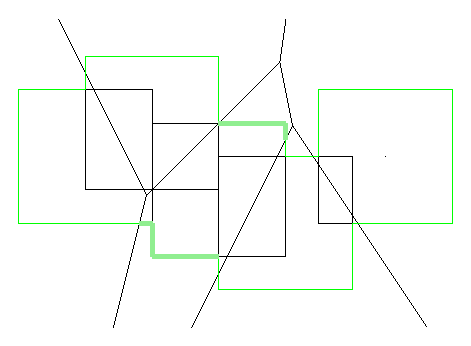
\includegraphics[scale=0.8]{3d/3d_perimeter_squares_truth}
    \caption{In green what we want}
    \label{fig:3d-inclusion-exclusion-squares-1}

    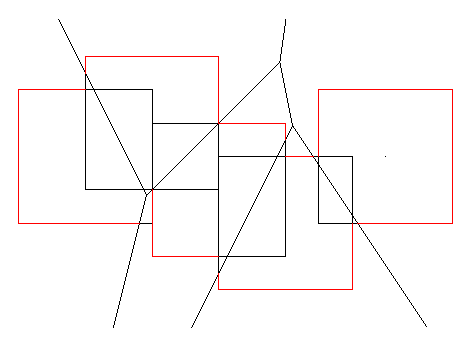
\includegraphics[scale=0.8]{3d/3d_perimeter_squares}
    \caption{In red what we actually compute}
    \label{fig:3d-inclusion-exclusion-squares-2}
\end{figure}

We see that there is a small difference between the two: our computation is just
an approximation.

% TODO: explain approximation

% {{{3 INCLUSION-EXCLUSION FORMULA
\subsubsection{Inclusion-exclusion formula}
% TODO

The inclusion-exclusion formula is a well known formula which describes the
indicator function of a union of sets: given a finite number of sets $ A = \{
A_1, \ldots, A_N \} $, we have:

$$ \indicator{\bigcup A_i} = \sum_{\emptyset \neq X \subseteq A} (-1)^{card X -
    1} \indicator{\bigcap X} $$

This formula can also be expressed using the notion of nerve as shown in
\cite{attali2007inclusion}. We defined the nerve of $ A = \{ A_x, x \in X \} $
to be the graph where an edge exists between $ x $ and $ y $ only if $ A_x \cap
A_y \neq \emptyset $.

Then, we can write the inclusion-exclusion formula as:

$$ \indicator{\bigcup A_x} = \sum_{\sigma \in Nerve(A)} (-1)^{\dim \sigma}
\indicator{\bigcap \sigma} $$

In our case, we get:

\begin{equation}
    \indicator{\bigcup B_N(p, r)} = \sum_{\sigma \in Nerve(B)} (-1)^{\dim \sigma}
    \indicator{\bigcap \sigma}
    \label{eqn:incl_excl_simplices}
\end{equation}

where $ B $ is the collection of all the balls $ B_N(p, r), p \in P $.

We will need the following definition:
\begin{definition}
    The $\alpha$-complex of a set of points $ X $ denoted by $ Del(X, \alpha) $
    is a subset of the Delaunay triangulation.

    For each simplex of the Delaunay triangulation, we can associate to it a
    characteristic radius: the radius of the smallest empty circle containing
    the simplex.

    Now, the $\alpha$-complex contains all the simplices of the Delaunay
    triangulation whose characteristic radii is smaller than $\alpha$.
\end{definition}

Now, we will approximate the equation \ref{eqn:incl_excl_simplices} by replacing $ Nerve(B)
$ by $ Del(P, r) $.

% TODO: explain why approximation

A question we can ask is: is the inclusion-exclusion formula still valid if we
replace $ Nerve(B) $ with $ Nerve(\{ B_N(p, r) \cap V(p, P), p \in P\}) $ ?

If we want to prove this assertion, we may use the technique used to prove the
inclusion-exclusion formula for union of balls.

The proof starts by defining the subcomplex $ L_p $ induced by a vertex $ p $.
We consider all the polyhedrons that contains $ p $ and we construct the nerve of
it. Formally, $ L_p = Nerve(\{ B_N(x, r), p \in B_n(x, r)\}) $.

Then, when we evaluate the indicator function at $ p $ of the union, we can
decompose it in two parts: simplices of $ L_p $ and the other ones.

\begin{align*}
    \indicator{\bigcup B_N(p, r)}(p) &= \sum_{\sigma \in L_p} (-1)^{\dim \sigma}
    \indicator{\bigcap \sigma}(p) + \sum_{\sigma \notin L_p} (-1)^{\dim \sigma}
    \underbrace{\indicator{\bigcap \sigma}(p)}_{= 0 \text{ since } p \notin
        \sigma} \\
    &= \sum_{\sigma \in L_p} (-1)^{\dim \sigma} \\
    &= \chi(L_p)
\end{align*}

Here, $ \chi $ is the Euler characteristic of $ L_p $.

Now, if we show that $ L_p $ is contractible (can be continuously deformed to a
point), we will get $ \chi(L_p) = 1 $. Obviously, we also have $
\indicator{\bigcup B_N(p, r)}(p) = 1 $ and we will conclude that the formula
\ref{eqn:incl_excl_simplices} is true.

We can use this argument to generalize this formula. If we suppose that there
exists $ r, r' $ such that: $ B(p, r) \subseteq B_N(p, r) \subseteq B(p, r') $,
then we have: $ K_p \subseteq L_p \subseteq K'_p $ where $ K_p $ (resp. $ K'_p $)
is the induced subcomplex of $ p $ in the simplicial complex defined by all the
balls $ B(p, r) $ (resp. $ B(p, r') $), $ p \in P $.

Then, we know that $ K_p $ and $ K'_p $ are either empty or contractible. We
want to deduce that $ L_p $ is either empty or contractible which will end the
proof.

% TODO: finish the proof

% {{{1 IMPLEMENTATION DETAILS
\section{Implementation details}

We used the same libraries as in the 2D case except for the rendering part, in
2D, we used custom \texttt{QWidget}. In this part, we choose to use an
\texttt{OpenGL} based renderer: \texttt{QGLViewer}.

For the first method, the Voronoi diagram is represented implicitly as a list of
halfspaces (the planes defining the boundary of the cell). Halfspaces are
computed using the Delaunay triangulation. Since the order traversal of the vertices
of the Delaunay triangulation is not, in general, be the same as the insertion
order, we need to associate an index to a point (using a simple
\texttt{std::map}).

For the two methods, we needed a way to compute intersection of halfspaces: for
the first one, we need to compute the intersection of a Voronoi cell and a
convex polyhedron and for the second one, we need to compute intersections of
convex polyhedra.

A convex polyhedron $ K $ represents the unit ball for the polyhedral norm
defined by $ K $. It is represented as a list of the normal vectors for each
facet. Using this representation, we can compute the translated polyhedron $
B_K(p, r) $ for a point $ p $ by saying that it is the intersection of the
following halfspaces: $ \forall n,~ n_x x + n_y y + n_z z - (p | n) - r \leq 0 $
where $ n $ is a normal vector of a facet.

In order to construct this intersection, we used the duality which allows us to
replace the computation of the intersection by the computation of the convex
hull (see \cite{preparata1979finding}) of the dual points: at each halfspace, we
can associate a dual point and conversely.

Programmatically, we compute this intersection in the following manner:
\begin{enumerate}
    \item Compute the dual points by remembering which point is associated to
        which plane
    \item Compute the convex hull of these points, it gives us a dual
        polyhedron. At each vertex, we associate the corresponding primal plane.
    \item To compute the primal polyhedron, we first compute the primal vertices
        which are the dual of the dual facets: each dual facet has at least 3
        vertices. We know the corresponding primal planes for these vertices.
        Then, the corresponding primal vertex is the intersection of these 3
        planes. Then, the primal facets are constructed by circulating around
        the dual vertices. Each time there is an edge between two dual vertices,
        there is an edge between the two corresponding primal vertices.
\end{enumerate}

Here is a simplified version of this algorithm:
\lstinputlisting[language=C++]{code/halfspace_intersection_with_dual_3.h}

Let's now explain in more details the integration of the automatic
differentiation tool.

\texttt{CGAL} has the particularity to make easy for the programmer to change
the number type by using the concept of a \emph{Kernel}. A \emph{Kernel} is a
class that describes how numbers are stored in memory, how we can construct
things (like points, planes, bisectors...) and how to evaluate predicates on
objects (collinearity test, coplanarity test, greater distance to a plane...).
There are multiple predefined kernels but we will quickly talk about two
particular ones. \texttt{Simple\_cartesian<NT>} is the most basic one: a number
will just be represented by \texttt{NT} and so it has inexact predicates
evaluation and inexact constructions.

\texttt{Exact\_predicates\_inexact\_constructions\_kernel} (in short
\texttt{Epick}) is a Kernel which use a technique called \emph{filtering} to
ensure the predicates are always evaluated in an exact manner. In short, the
predicate is the first evaluated in an inexact way using interval arithmetic.
Then, if the resulting interval does not contains zero, then a result can be
returned. Otherwise, the computation is done again using exact arithmetic which,
in all the cases, will give back an answer.

This is precisely the technique we used to use Automatic Differentiation with
\texttt{CGAL}, we used the Kernel: \texttt{Simple\_cartesian<AD>} where
\texttt{AD} is a class with two members: a value and a vector of derivatives.
It implements all the classical arithmetic operations and some mathematical
functions (\texttt{sqrt}, \texttt{atan2}...).

For example, the implementation of \texttt{sqrt} for AD looks like this:
\lstinputlisting[language=C++]{code/sqrt_AD.h}

The choice of \texttt{Simple\_cartesian} may seem inappropriate because the
constructions are inexact but it is enough for our applications.

Now, for the second method, we also needed a way to compute the $\alpha$-complex
of a set of points. This has been done using the \texttt{Alpha\_shapes\_3} class
of \texttt{CGAL}.

% TODO

% {{{1 EXPERIMENTS
\section{Experiments}

% TODO

We compare the two different methods using various polyhedrons as base and
various point clouds.

We can choose for the polyhedron a sufficiently discretized sphere. We expect
the result to be the same as in the 2D case: gradients oriented like the outward
normal with a norm proportional to the mean curvature.

The figures \ref{fig:3d-mean-curvature-sphere-cube} give an example where the
point cloud is a sphere and the polyhedron is a cube.

\begin{figure}[h]
    \centering
    \begin{minipage}{0.32\linewidth}
        \centering
        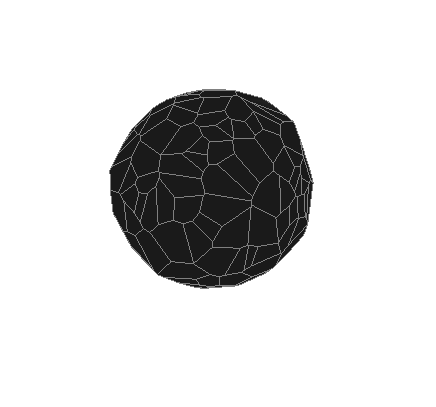
\includegraphics[scale=0.3]{3d/sphere-polyhedron-200}
        \subcaption{Discretized sphere with 200 planes}
    \end{minipage}
    \begin{minipage}{0.32\linewidth}
        \centering
        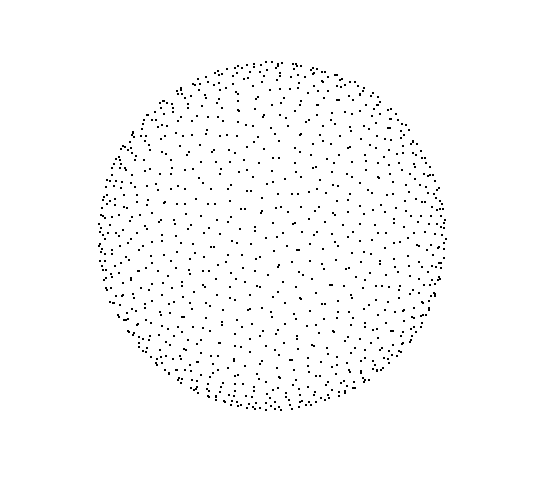
\includegraphics[scale=0.3]{3d/sphere-1000}
        \subcaption{Initial point cloud: 1000 points on a sphere}
    \end{minipage}
    \begin{minipage}{0.32\linewidth}
        \centering
        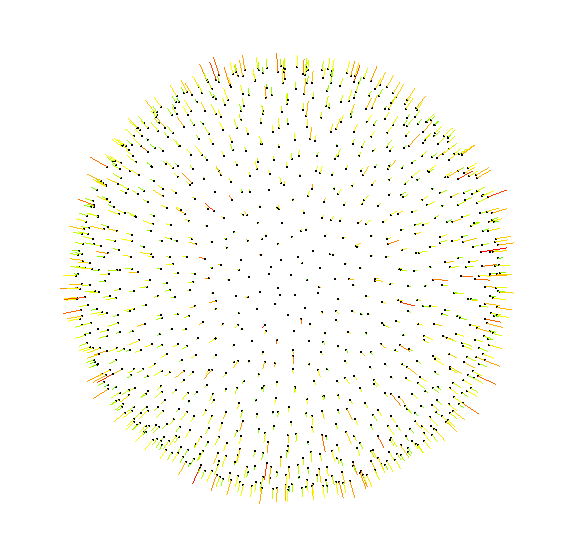
\includegraphics[scale=0.3]{3d/sphere-sphere-1000-05}
        \subcaption{Gradients of the volume}
    \end{minipage}
    \caption{Sphere / cube}
    \label{fig:3d-mean-curvature-sphere-cube}
\end{figure}
We remark that the gradients are oriented like the outward normals.

We also did some experiments for checking the convergence of the flow.

The figures \ref{fig:3d-flow-sphere-cube} give an example where the point cloud
is a sphere and the polyhedron is a cube.

\begin{figure}[h]
    \centering
    \begin{minipage}{0.32\linewidth}
        \centering
        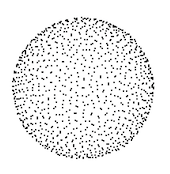
\includegraphics[scale=0.4]{3d/sphere-cube-0}
        \subcaption{Initial sphere with 1000 points}
    \end{minipage}
    \begin{minipage}{0.32\linewidth}
        \centering
        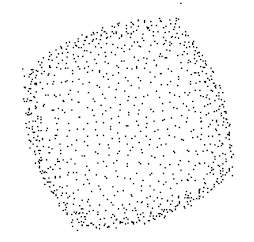
\includegraphics[scale=0.4]{3d/sphere-cube-10}
        \subcaption{After 10 iterations}
    \end{minipage}
    \begin{minipage}{0.32\linewidth}
        \centering
        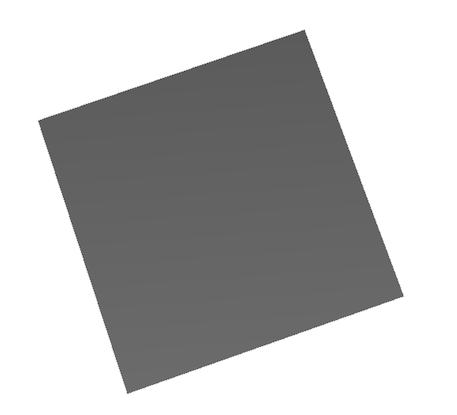
\includegraphics[scale=0.3]{3d/sphere-cube-cube}
        \subcaption{Shape of the cube}
    \end{minipage}

    \caption{Flow of a sphere under a cube}
    \label{fig:3d-flow-sphere-cube}
\end{figure}

% TODO:
% - description des différentes méthodes + comparaison
% - résultats

% vim: set spelllang=en :
% {{{1 THEORY
\section{Theory}

In this section, we will show that the function that we are trying to minimize
is not the volume of the Minkowski sum but another functional close to the
first one.

We will need the definition of the radial function of a convex set:

\begin{definition}
    For a convex set $ K $, we define the radial function $ \rho_K $ by:
    $$ \rho_K(x) = \sup \{ r \in \R,~rx \in K \} $$
\end{definition}

Let us denote by $ A $ the following functional:

$$ A(S) = \int_S \int_{-r \rho_K(-\vec{n}_S(x))}^{r \rho_K(\vec{n_S}(x))} J_\phi(x)
dt dx $$

where $ K $ is the chosen convex polyhedron and $ S $ the underlying smooth
surface we sample points on.

$ \phi $ is the usual change of variable: $ \phi(x) = x + t \vec{n}_S(x) $ for $
x \in S $ and $ t \in [-r \rho_K(-\vec{n}_S(x)), r \rho_K(\vec{n_S}(x)) ] $.

We have, in 3D, using the lemma \ref{lemma:diffeo}:

\begin{align*}
    A(S) &= \int_S \int_{-r \rho_K(-\vec{n}_S(x))}^{r \rho_K(\vec{n_S}(x))}
    \left[ 1 + (\kappa_1(x) + \kappa_2(x)) t + \kappa_1(x) \kappa_2(x) t^2
    \right] dt dx \\
    &= \int_S (r \rho_K(\vec{n_S}(x)) + r \rho_K(-\vec{n_S}(x))) dx + O(r^2)
\end{align*}

Now, if $ K $ is symmetric, i.e. if $ x \in K $ then $ -x \in K $ which implies
that $ \rho_K(\vec{n_S}(x)) = -\rho_K(-\vec{n_S}(x) $, then we get:

$$ A = 2r \int_S \rho_K(\vec{n}_S(x)) dx + O(r^3) $$

So:

$$ \frac{1}{2r} A = \int_S \rho_K(\vec{n}_S(x)) dx + O(r^2) $$

Then, the functional we minimized is $ A $ and not the volume if the Minkowski
sum.

